\chapter{Background}\label{Introduction}
\section{SQL}\label{theory}
Turing completeness of SQL:1999
\subsection{Declarativity and the Query Planner}

\subsection{User Defined Functions}
Possible Languages, (Im)possible optimizations

\subsection{Evaluation of \texttt{WITH RECURSIVE}}
$$
q_0 ~\cup ~\underbrace{q_r(q_0)}_{q_1} ~\cup~ \underbrace{q_r(q_1)}_{q_2}~ \cup~\underbrace{q_r(q_2)}_{q_3}~ \cup ~\hdots ~ \cup ~ \underbrace{q_r(q_n)}_{= \emptyset}
$$

Recursive evaluation is composed of an nonrecursive basecase and an recursive case that references the results of the previous iteration.
Stop when no new results are produced
https://www.postgresql.org/docs/10/static/queries-with.html

\section{Recursion}
\subsection{Types of recursive functions}
\subsection{Iterative solving of recursive functions}
\subsection{Dynamic Programming}
\subsection{Memoization}

\begin{figure}
    \centering
    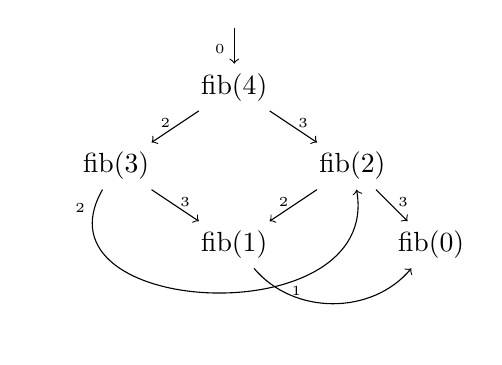
\begin{tikzpicture}
% nodes
\node (f4)     at (2.5, 2) {fib(4)};
    \node (f3) at (1, 1) {fib(3)};
        \node (f1) at (2.5, 0) {fib(1)};
    \node (f2) at (4, 1) {fib(2)};
        \node (f0) at (5, 0) {fib(0)};
% arrows
\draw[<-] (f4) -- node[pos=0.4, left, label distance=5mm]{\tiny{0}} +(0, 0.75);

\draw[->] (f4) -- node[pos=0.4, left, label distance=5mm]{\tiny{2}} (f3);
\draw[->] (f4) -- node[pos=0.4, right, label distance=5mm]{\tiny{3}} (f2);

    \draw[->, bend right=100, out=240, looseness=1.5] (f3) to node[pos=0.05, left, label distance=5mm]{\tiny{2}} (f2);
    \draw[->] (f3) -- node[pos=0.4, right, label distance=5mm]{\tiny{3}} (f1);
    \draw[->] (f2) -- node[pos=0.4, left, label distance=5mm]{\tiny{2}} (f1);
        \draw[->, bend right=50] (f1) to node[pos=0.2, right, label distance=5mm]{\tiny{1}} (f0);
    \draw[->] (f2) -- node[pos=0.4, right, label distance=5mm]{\tiny{3}} (f0);
\end{tikzpicture}
    \caption{Callgraph with memoization, The callstack-tree becomes a Directed Acyclic Graph (DAG). Each node represents an invocation and each outgoing edge a new callsite. Because of memoization, evaluation of equal invocations is performed only once, ie. they have the same descendants.}
    \label{fig:fib_callstack_memoization}
\end{figure}

\section{Operational Semantics}\label{SOS}